\RequirePackage{filecontents}
\begin{filecontents}{BIBLIOGRAPHY.bib}
@Article{balk_2010,
  title={Regression-type problems under zero median noise},
  author={Balk, PI},
  booktitle={Doklady Mathematics},
  volume={81},
  number={1},
  pages={142--145},
  year={2010},
  organization={Springer}
}

@book{product_1995, 
 title={Summation and Product Notation},
 author={I.S.U.M.D},
 organisation={Illinois State University Mathematics Department},
 url={http://math.illinoisstate.edu/day/courses/old/305/contentsummationnotation.html},  
 journal={Summation and Product Notation}, 
 year={1995}}
 
 @inbook{matthews_1998, 
 place={Berlin}, 
 title={Vector calculus}, 
 publisher={Springer}, 
 author={Matthews, P. C.}, 
 pages={45--48},
 year={1998}}


@inbook{stewart_2008_int, 
 place={Belmont, CA}, 
 title={Calculus: early transcendentals}, 
 publisher={Thomson Brooks/Cole}, 
 author={Stewart, James}, 
 pages={950--1021},
 year={2008}}
 
 @inbook{stewart_2008_deriv, 
 place={Belmont, CA}, 
 title={Calculus: early transcendentals}, 
 publisher={Thomson Brooks/Cole}, 
 author={Stewart, James}, 
 pages={878--891},
 year={2008}}
 
@book{cromwell_1999, 
 place={Cambridge}, 
 title={Polyhedra}, 
 publisher={Cambridge University Press}, 
 author={Cromwell, Peter R.}, 
 year={1999}}
 
 @article{Weisstein_2014,
author = {Weisstein, Eric W.},
publisher = {From MathWorld--A Wolfram Web Resource},
title = {Dimension},
year = {2014},
url = {http://mathworld.wolfram.com/Dimension.html},
}

@book{kelley_1995, 
 place={New York}, 
 title={General topology}, 
 publisher={Springer}, 
 author={Kelley, John L.}, 
 year={1995}}
 
 @article{Plackett_1950,
author = {Plackett, R. L.},
journal = {Biometrika.},
number = {1-2},
pages = {149-157},
title = {Some Theorems in Least Squares},
volume = {37},
year = {1950},
}

@incollection{Ross_2007,
author = {Sheldon M. Ross},
booktitle = {Introduction to probability models (9th ed)},
publisher = {Academic Press},
title = {2.4 Expectation of a random variable},
year = {2007},
}

\end{filecontents}
\documentclass[11pt,a4paper]{article}
\usepackage{graphicx}
\graphicspath{ {images/} }
\usepackage{natbib}
\usepackage[rightcaption]{sidecap}
\usepackage{svg}
\usepackage{transparent}
\usepackage{xcolor}
\usepackage{relsize}
\usepackage{amsmath}
\usepackage{amsfonts}
\usepackage[margin=2cm]{geometry}
\usepackage{fancyhdr}
\usepackage{enumitem}
\pagestyle{fancy}
\usepackage{float}
\usepackage{cancel}
\usepackage{subfig}
\usepackage{multirow}
\usepackage[utf8]{inputenc}

\numberwithin{equation}{subsection}

\title{Deriving an Alternative Data Approximation Method to Be Used in Non-typical  Circumstances}
\date{\today}

\begin{document}
%TITLE
\begin{titlepage}
\begin{center}
IB Mathematics Higher Level Internal Assessment on Statistics 
\\ 
\rule{\textwidth}{0.25pt}
\linebreak
\Huge{Deriving an Alternative Data Approximation Method to Be Used in Non-typical  Circumstances}
\rule{\textwidth}{0.25pt} \\
[15cm]
\large {David Simon Tetruashvili} \\

\end{center}
\end{titlepage}
\newpage
%TITLE END
\pagenumbering{0}
%TOC
\tableofcontents
\pagenumbering{arabic}
\newpage
%TOC END

%Body
\section{Introduction}
In both physics and mathematics practical work has as much value to humanity as theoretical does. In my school career there have been countless labs, practicals and experiments. I have come to notice that during all of these labs, practicals and experiments in any field, if the lab, practical or experiment is quantitative, the data gathered, almost always, has to be approximated into some kind of functional dependence to be of further use. This made me wonder how do these approximations work; how does a calculator know what the best fit line is? Further more, I've also noticed that in all of these practicals, the method of approximation that my classmates and I  are told to use (and the one that is most commonly used) is the so called Least Square Method (LSM). What does it imply? What logic does it use to approximate? When does it work best, and when does it not work at all? I've grown concerned about the validity of my practical results that I have used in the past. What if the approximation had large errors? How big can those errors be? \\
\\
In this IA I aim to suggest an alternative method/algorithm of approximation, one that performs better in certain situations, in which the LSM does not. I will do so by deriving the formula for the optimal parameter(s) of a given functional dependence. Then I will use self-written software to (via the formula derived) calculate trials in which it is shown that the method that is suggested in this IA, indeed works better in given circumstances when compared to LSM. 
\section{Mathematical Background}
Because of the nature of IB Mathematics IAs, the mathematics in this written work extend from the IB syllabus. Some notations, concepts, and calculations have to be explained. 

\subsection{Notations}
During the IB Math HL program, students learn about vectors. 2D-Vectors usually have only magnitude and direction, however, a vector can only be 3D, or even 4D. Essentially, so long that a single value has multiple parameters (components) it is a vector in the same number of dimensions as there are parameters. In this IA, all vectors will be denoted with the variable $c$, be it with some indexes or accents, as long as a variable has $c$ in its core, it is a vector. Note that this is just a notation that I will use only in this paper. In addition, to save real estate, no vertical vector notation will be used, instead I will use the so called ordered set notation of a vector in the form of $c=(c_{1},c_{2},\dots)$. Where the vector $\dot{c}$ is in real coordinate space\footnote{\cite{kelley_1995}}; This allows several real variables to be treated as one, single variable. The notation $\boldsymbol{R}^{m}$ describes the dimension of space. I.e. $\boldsymbol{R}^{1}$ is one-dimensional space, $\boldsymbol{R}^{2}$ two-dimensional, and so on.\footnote{\cite{Weisstein_2014}}. \\
\\
Another new to IB notation in this IA is the product notation:
\begin{gather*}
\prod\limits_{i = m}^{n} x_{i} = x_{m} \cdot x_{m+1} \cdot \  \cdots \  \cdot x_{n-1} \cdot x_{n}.
\end{gather*}
This essentially works in much of the same way the familiar summation notation we use in class(using the Greek capital letter sigma), except that instead of summing values, it multiplies them (and uses Greek the capital letter pi) \footnote{\cite{product_1995}}.
\subsection{Concepts}
Derivatives are an essential part of the IB curriculum. But when it comes to functions with multiple variables (like in this IA), their derivative is taken differently. First off, the derivative of such functions is called a partial derivative. Denoted using a stylized symbol $\partial$, it is the derivative of a function with multiple variables, with respect to one of them, when others are held constant \footnote{\cite{matthews_1998}, pages 45-48} \footnote{\cite{stewart_2008_deriv}, pages 878-891}. The following example will explain this further:\\
\\
Find the local minimum of function $z$ with multiple variables:
\begin{gather*}
z = f(x,y) = 5(2x-3)^{2} + 4(4y+1)^{2}
\end{gather*}
Without calculating anything, we see that the minimum of this function occurs when $x= \frac{3}{2} $,$ y= -\frac{1}{4}$.
\begin{gather*}
\text{( Now expand this function )}\\
z = 20x^{2} + 64y^{2} -60x + 32y +49
\end{gather*}
Now according to normal method of finding a minimum of a function, we equate, in this case, its partial derivatives (one with respect to $x$, the other to $y$) to zero and solve for $x$ and $y$.
\begin{eqnarray*}
\frac{\partial f(x,y)}{\partial x}  &=&  40x-60 = 0 \rightarrow x = \frac{60}{40}=\frac{3}{2}\\
\frac{\partial f(x,y)}{\partial y}  &=&  128y-32 = 0 \rightarrow y = -\frac{32}{128}=-\frac{1}{4}
\end{eqnarray*}
Voilà, the partial derivatives gave us the answer as well.\\
\\
But as much as derivatives a essential, so are integrals. This IA invokes the use of something called multiple integrals. These are basically integral an of integral, where again a function with multiple variables is in question \footnote{\cite{stewart_2008_int}}. I.e. a double (two-multiple) integral of some two-variable function $g(x,y)$ is denoted as such:
\begin{gather*}
\int \int g(x,y) \mathrm{d}x\mathrm{d}y
\end{gather*}
Yet again let's employ an example: \\
Find the area of the shaded region\\
\begin{center}
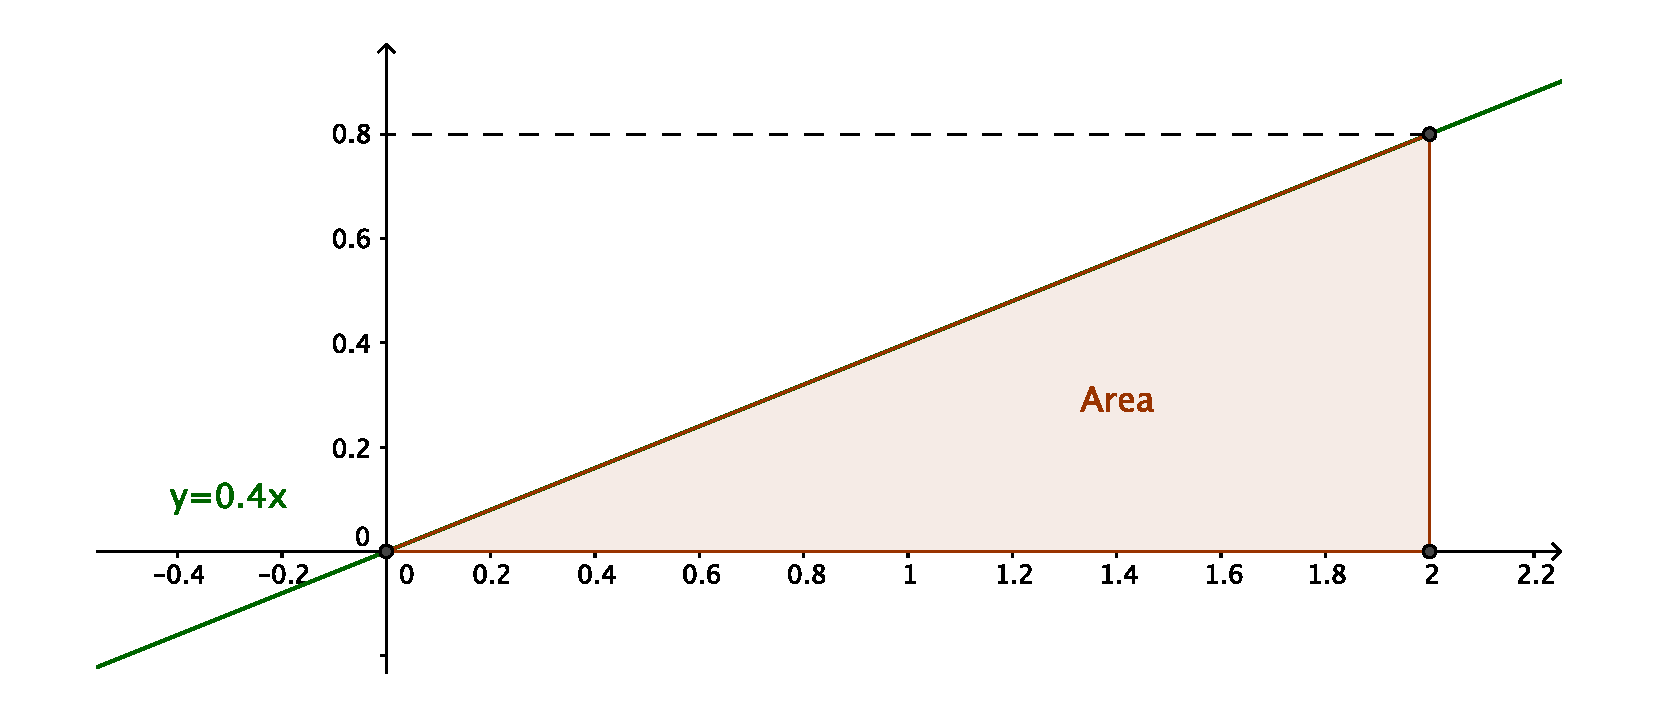
\includegraphics[scale=0.4]{pic-multiexample}
\end{center}
Obviously, $$A=\frac{1}{2}\cdot 2 \cdot 0.8 = 0.8.$$ Granted, the following method is very unnecessary (and this problem doesn't even require a multiple integral), but for the sake of explanation, let's employ multiple integrals as well.
\begin{gather*}
A = \underbrace{\int\limits_{0}^{2}}_{\text{(against } x\text{)}} \underbrace{\int\limits_{0}^{0.4x}}_{\text{(against } y\text{)}} \mathrm{d}x \mathrm{d}y =  \int\limits_{0}^{2} \mathrm{d}x \cdot \left[ y \right]_{0}^{0.4x} =  \int\limits_{0}^{2} \mathrm{d}x \cdot  \left[ 0.4x - 0 \right] = \int\limits_{0}^{2} \mathrm{d}x \cdot 0.4x = 0.4 \int\limits_{0}^{2} x\mathrm{d}x = \\
0.4 \cdot \left[ \frac{x^{2}}{2} \right]_{0}^{2} = 0.4 \cdot \left[ \frac{2^{2}}{2} - \frac{0^{2}}{2} \right] = 0.4 \cdot 2 = 0.8.
\end{gather*}
And, again, the answer is the same. Now with these mathematical concepts explained we formulate the problem of this IA.

\section{Formulation of the Problem}

A function is one of the most known mathematical objects. An important task which has practical applications, is the approximation of a function or relationship based on some information known about the function or relationship in question. This information may either be determinate or statistical. An example of a determinate piece of information about function $f(x)$ is its range (or the possible values this function may have) on a given interval $[\alpha,\beta]$. Example of a statistical information may be the law of distribution of random errors $\xi_{i}$ in approximate values $\tilde{y}_{i} = f(x_{i})+\xi_{i}$ of the function, which in turn can describe a certain physical process (change of temperature over time, for example). In practice, a number $n$ of points $x_{i}$ can be obtained as results of some kind of physical experiment. Where in this case, the approximation of function $f(x)$ only makes sense if the this function is described by a finite number $m<n$ of parameters (coefficients) $c_{j}$, where the true values of said parameters will be denoted as $\dot{c}_{j}, \ j=1,2,\dots,m.$ \\
\\
This Internal Assessment will focus on the estimation of parameters of the function \footnote{Here, because the vector $\dot{c}$ has $m$ parameters (components), it will also be in $m$-dimensional space.}
\begin{equation}
y = f(\dot{c},x_{i}),\quad \dot{c} \in \boldsymbol{R}^{m},\quad x \in [\alpha,\beta],\quad \dot{c} = (\dot{c}_{1}, \dot{c}_{2},\dots,\dot{c}_{m}) \label{301}
\end{equation}
based on its approximate values
\begin{equation}
\tilde{y}_{i} = f(x_{i})+\xi_{i}, \quad i=1,2,\dots,n ,
\end{equation}
when additionally it is also known, that: 1. vector $\dot{c} = (\dot{c}_{1}, \dot{c}_{2},\dots,\dot{c}_{m})$ belongs to a given limited set $D$, like for example a parallelepiped in $\boldsymbol{R}^{m}$ dimensions; 2. $\xi$ is a limited continuous random value; the median of which $Med(\xi)$ is equal to zero. \\
\\
Judging by references in scientific works that I read while researching for this IA [citations needed], the most popular linear model of a studied relationship is
\begin{equation}
f(\dot{c},x)= \sum\limits_{j=1}^{m} \dot{c}_{j} \phi_{j}(x), \label{functionform}
\end{equation}
specifically in polynomial form, when
\begin{equation}
\phi_{1}(x)\equiv 1; \quad \phi_{j}(x)=x^{j-1},\quad j=1,2,\dots,m.
\end{equation}
\\
In practice, it is often the case when it is not only necessary to estimate the parameters of a function, but identifying the type (structure) of this function is needed as well. In other words, a finite number $L$ of alternative structures is given
\begin{equation}
f_{l}(c;x), c \in \boldsymbol{R}^{m(l)}, \quad l=1,2,\dots,L,
\end{equation}
and it is necessary to identify to which of $L$ structures of function $f_{l}(c;x)$ belongs the function $f(\dot{c},x)$, and after that estimate the vector $\dot{c}$ of its parameters. In our school program, the class has encountered one such task, when it was said to find out if we were dealing with a linear or exponential relationship, be it in either physics or math. However, then, this problem was solved using the exact (or near to exact) values of both of the relationships, so it was easy to distinguish them. \\
\\
There are countless papers dedicated to the approximation of functions based on their approximate values (in practice - experimental data). Usually, in such papers the consensus is to use a certain condition. This condition is to assume that the mathematical expectancy of error is equal to zero \footnote{\cite{Plackett_1950}}.
\begin{equation}
E(\xi)=0
\end{equation}
 However, in this IA this condition will not be used. Here instead of the condition of mathematical expectancy of error $\xi$ being equal to zero, I will assume that the median of the same error $\xi$ being equal to zero, 
\begin{equation}
Med(\xi)=0
\end{equation}
specifically when the algorithm of evaluation of the parameters of the function is based on ideas from the \textit{method of least squares}. \\
\\
I justify my interest to the condition $Med(\xi)=0$ by the case when the traditional condition $E(\xi)=0$ is unachievable. This happens when measurements are taken close to one of the natural limits of the physical relationship being measured. An example of such natural limit is the inability of some magnitude, such as weight, to be negative. In this case, the absolute value of the error made, can only be large (with respect to other errors made) in the \textit{same sign}, either positive or negative. Figure \ref{fig:graph-nl} shows an example of this graphically.
\begin{figure}[h!]
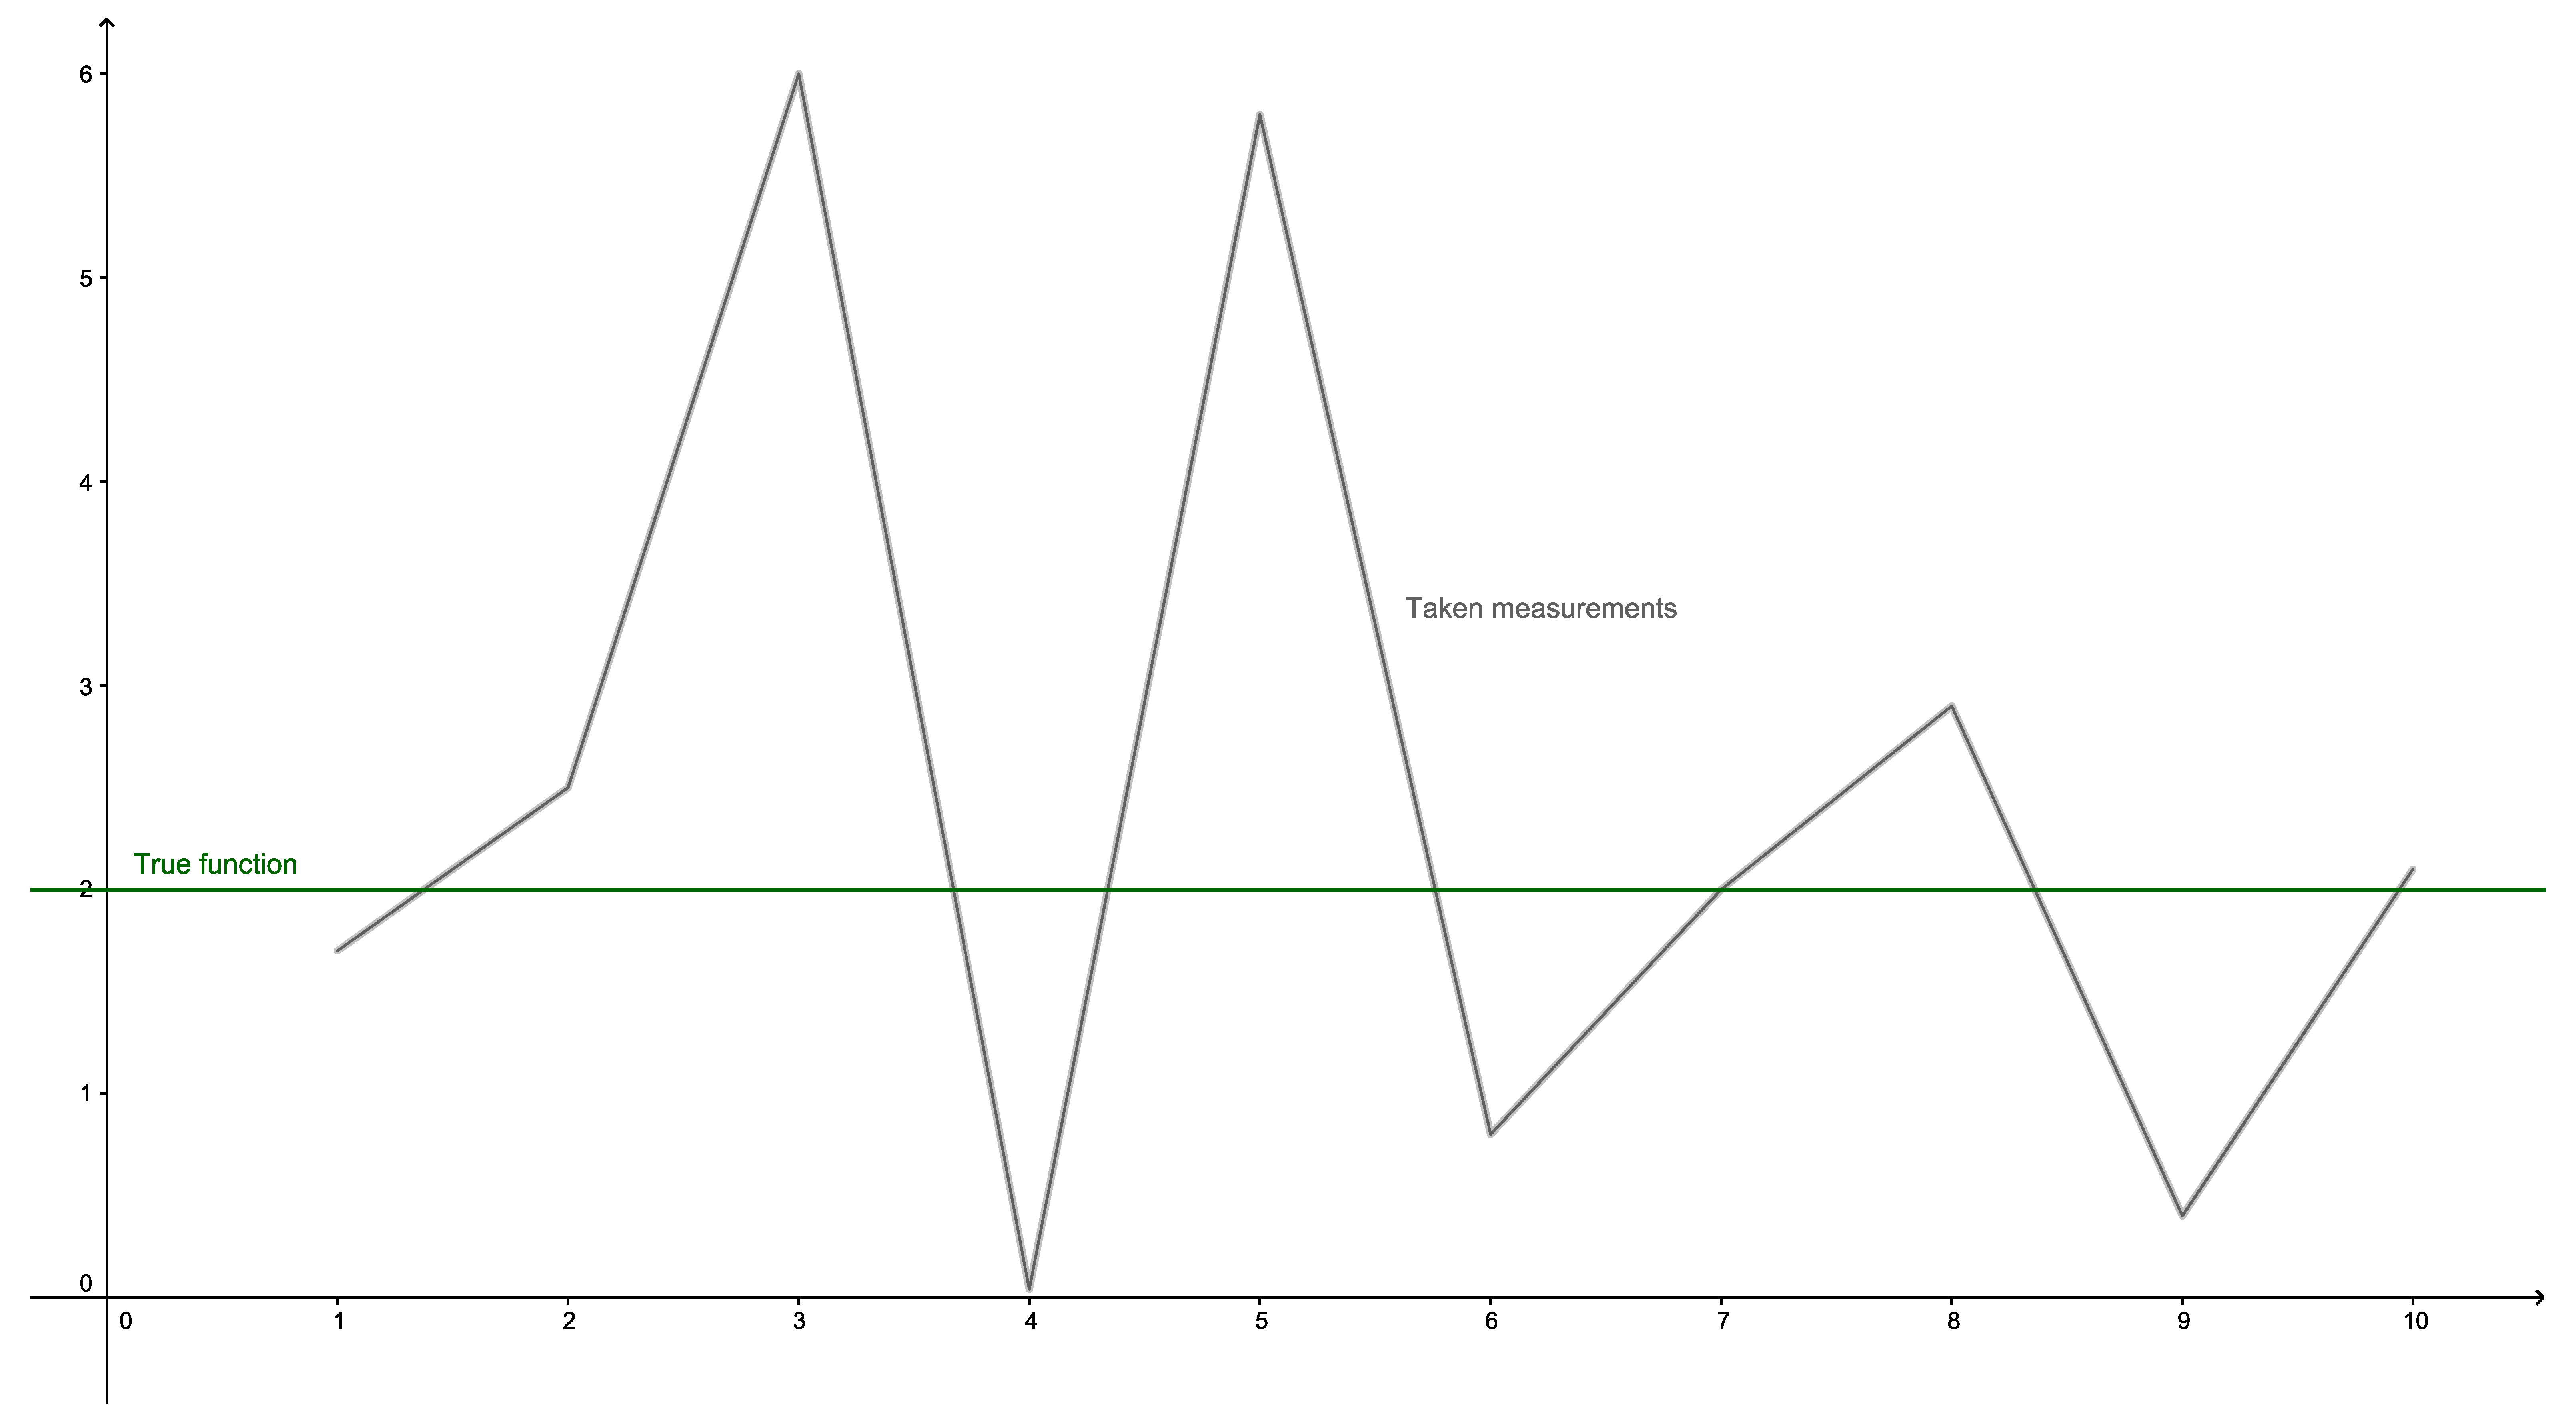
\includegraphics[scale=0.1]{pic-naturallimits}
\centering
\caption{Graphical representation of a case where $E(\xi)=0$ does not work effectively.}
\label{fig:graph-nl}
\end{figure}
\\
I want to bring attention to the fact, that the argument that this kind of measurement could be withdrawn by human intervention, is invalid for 2 reasons: 1. Any such withdrawal usually leads to loss of information. 2. In cases where the experiment requires high-capacity data collection human intervention may not be possible.\\
\\
Speaking of the errors, what is meant is not only error that was produced by a faulty measurement, but also any error caused by some factor that was either omitted or unaccounted for in function $f(x)$. Even though both conditions $E(\xi)=0$ and $Med(\xi)=0$ are not special cases of each other,it could be argued that from a point of view of solving practical problems, the condition $Med(\xi)=0$ is the more broad of the two (as in, it is easier to meet). The only requirement for meeting this condition is $P(\xi)>0$ is 0.5.  Hence the condition $Med(\xi)=0$ allows for some comparatively large random values of error $\xi$ to be on one side of the true function and not on the other, without the approximation to be significantly affected by those large values, unlike the condition $E(\xi)=0$. With condition $Med(\xi)=0$ the approximation can account for large peaks in values of $\xi$.\\
\\
As mentioned before, the aim of this AI is as follows. To create an algorithm, capable of estimating the parameters of a functional dependence whose structure is known, accurately,  and to securely give an estimate to the accuracy of the calculated approximate values of the functional dependence. \\
\\
Its clear that the quality of the solution of this problem is dependant of an array of factors, which include: 1. the ratio between the number $n$ of measurements $\tilde{y}_{i}$ and the number $m$ of estimated parameters $\dot{c}_{j}$. 2. the intensity of error $\xi_{i}$ 3. the number of $L$ alternatives, and more importantly, the degree of similarity of functions $f_{l}(c;x)$. This means that to confirm my theoretical reasoning, quite an ambitions computational experiment is required. I will proceed with the necessary calculations using custom software. 

\section{Algorithm}

Approximation of a functional dependence taking this new condition $Med(\xi)=0$ in mind, has been looked at in mathematics (like for example in Regg-Med-Noise, [citation needed]). It is believed that in this case it is necessary to minimize the sum of absolute values of deviations of the modelled dependence $f(c^{*},x)$ from the unknown true function $f(\dot{c},x)$, where $c^{*}$ is the found optimal value of  vector $c$. This method is referred to as the Least Absolute Deviations (LAD). However, through my research I have found no methods of estimating LAD's accuracy. What value does an optimization method have if there is no way to determining the error it made? In addition, LAD does not presume the existence of priori limitations on the vector $\dot{c}$. And i must ask the question: What happens if the vector of parameters $c^{*}$, providing the minimum of the sum of modulus of errors, does not belong to the set $D$? \\
\\
It is clear, that in every separately taken case (run of an algorithm), the factual accuracy of the model solution (when the true function is known) cannot serve as either a comparative evaluation of two competing algorithms, nor criteria of effectiveness of any given algorithm. It is also clear, that if all, or close to all errors $\xi_{i}$ have the same sign (the condition $Med(\xi)=0$, although, the condition $E(\xi)=0$ as well, allow this, be it with a small probability), then neither method will give any good solutions. And also, with a certain 'layout' of errors $\xi_{i}$, a theoretically more sound method might by change give a worse solution that a less sound one. So, when estimating the effectiveness of a method, it is necessary to rely on average results of some number of random solutions. In conjunction with this, the idea lies in the fact that for the quality of constructed approximation $f(c^{*},x)$ to $f(\dot{c},x)$, I take the mathematical expectation \footnote{\cite{Ross_2007}}

\begin{equation}
E(\rho(c^{*},\dot{c}))= \int\limits_{D}P(c)\rho(c^{*},\dot{c})\mathrm{d}c_{1}\mathrm{d}c_{2}\dots \mathrm{d}c_{m}, \quad c = (c_{1},c_{2},\dots,c_{m}) \label{Erho}
\end{equation}
of proximity (distance) $\rho(c^{*},\dot{c})$ of function $f(c^{*},x)$ from $f(\dot{c},x)$ where in the role of distance $\rho(c^{*},\dot{c})$, one could take on of the functions
\begin{eqnarray}
\rho_{1}(c^{*},c) &=& \sum\limits_{j=1}^{m} \left| c_{j}^{*}-c_{j} \right| \label{rho1}\\
\rho_{2}(c^{*},c) &=& \sum\limits_{j=1}^{m} \left( c_{j}^{*}-c_{j} \right)^{2} \label{rho2}\\
\rho_{3}(c^{*},c) &=& \sqrt{\frac{1}{n}\sum\limits_{i=1}^{m} \left( y_{i}-f(c^{*},x_{i}) \right)^{2}} \label{rho3}
\end{eqnarray}
In solving the problem, that I have above labelled as 'aim-minimum', criteria (\ref{Erho}) was considered in article called \textit{'Reggression-type Problems under Zero Median Noise'}(from now on being refered to as 'Regg-Med-Noise') \footnote{\cite{balk_2010}}. Looking ahead, I say that I will suggest a more constructive algorithm than the one occurring in Regg-Med-Noise. I want to note that the problem that I have above labelled as 'aim-maximum' was not looked at in the mentioned paper. \\
\\
The probability density function $P(c),\  c \in D$ where $c$ is a vector that could be the unknown true vector $\dot{c}$, that (the function) appears in the $m$-multiple integral (\ref{Erho}), can be constructed on the basis of the formula of the binomial distribution of a random value [citation needed]. In fact, let's say: $c \in D$ is one of the vectors which claims that it is the unknown true vector $ \dot{c}$ from function (\ref{functionform}); $q_{i}$ are the elements of the sequence
\begin{equation}
q_{1}(c)=\tilde{y}_{1}-f(c,x_{1}),\ q_{2}(c)=\tilde{y}_{2}-f(c,x_{2}), \dots, \ q_{n}(c)=\tilde{y}_{n}-f(c,x_{n}); \label{sequence}
\end{equation}
where $q$ is a discreet random value, that can assume values
\begin{equation}
r=r(c)=\sum\limits_{i=1}^{n-1} \delta_{i}(c), \label{eq-values-of-q}
\end{equation}
where
\begin{equation}
\delta_{i}=\delta_{i}(c)=
\begin{cases} 
      1, \mathrm{if} \quad q_{i}(c)q_{i+1}(c)<0\\
      0, \mathrm{if} \quad q_{i}(c)q_{i+1}(c)\geq 0
   \end{cases}
\end{equation}
In meaningful terms, the value of $r$ is the number of transitions of sign of the elements of  (\ref{sequence}). Where $r \in [0,n-1]$. If it truly happens that $c=\dot{c}$, then the values of $q_{i}$ would be nothing but the errors $\xi_{i}$, and by the condition $Med(\xi)=0$ the probabilities $p_{r}$ of events $q = r$ could be written as
\begin{equation}
p_{r}= \frac{\binom {n-1}r}{2^{n-1}}, \quad r = 0,1,\dots,n-1. \label{priori}
\end{equation}
Lets move on from discussing the question of the transition of sign with some one vector $c$, to the analysis of this situation with regards to the whole set $D$. Say that there exists a partitioning of set $D$ into a family of sub-sets $D_{1},D_{2},\dots,D_{n}$ such that the elements (in this case vectors $c$) of sub-set $D_{r}$ provide the same number $r-1$ of transitions of sign of elements of (\ref{sequence}). Note that here the sub-sets $D_{r}$ will take the form of $m$-dimensional polyhedrons \footnote{In geometry, a polyhedron is a solid in three (in this case $m$) dimensions with flat polygonal faces, straight edges and sharp vertices. A polyhedron is said to be convex, if any two points within it can be connected by a line segment with this segment also being within the polyhedron. \cite{cromwell_1999}} as they are in $m$-dimensional space. In this way, the priori probability that the unknown true vector $\dot{c} \in D_{r}$ in given by (\ref{priori}). However, in any separate case, some of the sub-sets $D_{r}$ could be empty, meaning  that with some vectors of parameters $c \in D$, the number of transitions of sign of (\ref{sequence}) will not equal the given value of $r$ (any one can make sure of this by trying to draw a line which would crossed a given poly-line by guess, in such way that all of the endpoints of this poly-line turned out to be on either side of the guessed line). The priori probabilities $p_{r}$ that the unknown true vector $\dot{c}$ is in one of the non-empty sub-sets $D_{r}$ can be recalculated to the posteriori probabilities $p_{r}^{*}$. Let's define $I$ as the set of the numbers of all the non-empty sub-sets $D_{r}$. Then
\begin{equation}
p_{r}^{*}= 
\begin{cases} 
		\frac{p_{r}}{\sum\limits_{s \in I}p_{s}}, \quad r \in I.\\
		0, \quad r \in \{ 0,1,\dots,n-1 \} \setminus I
\end{cases}
\end{equation}
Because in our case the vectors $c$, are those that could be the true vector $\dot{c}$, are continuous values, and not discreet ones, then to use formula (\ref{Erho}) we must proceed from estimates $p_{r}^{*}$ of the probabilities of event $\dot{c} \in D_{r}$ to estimates $p_{r}^{*}(c), c \in D_{r}$, of a probability density function. As there is no information  which would allow me to somehow rank/sort the 'preference' of vector $c$ in the bounds of each sub-set $D_{r}$, it is logical to assume uniform distribution
\begin{equation}
P_{r}^{*}(c)=\frac{p_{r}^{*}(c)}{\mu(D_{r})}, \quad r \in I,
\end{equation}
where $\mu(D_{r})$ is the measure (analogous to the volume) of sub-set $D_{r}$ in $\boldsymbol{R}^{m}$ dimensions. \\
\\
Therefore (\ref{Erho}) becomes
\begin{equation}
E(\rho(c^{*},\dot{c}))=\sum\limits_{r \in I} \frac{p_{r}^{*}(c)}{\mu(D_{r})} \int\limits_{D_{r}}\rho(c^{*},\dot{c})\mathrm{d}c_{1}\mathrm{d}c_{2}\dots \mathrm{d}c_{m} \label{mathexpectancy}
\end{equation}
where $\int_ {D_{r}}(\bullet)$ is a laconic (short) notation of a multiple integral (in this case a $m$-multiple integral). In the general case, such as this one, the limits of integration of each univariate integral depend on variables, based on which the integration of the external integral relative to the given univariate integral is carried out \footnote{\cite{stewart_2008_int}}. (Refer to the example in section 2). This significantly complicates the calculation of these multiple integrals. Yet again, looking ahead, I want to note that in the algorithm created, integration is carried out on multidimensional parallelepipeds, when the limits of integration of each integral remain constant. \\
\\
\begin{subsection}{Illustrative example}
For it to be clear, that the following bulky equations lead to success, let's consider an illustrative example, where $m=1$ (i.e. the vector $\dot{c}$ is a scalar value), $y=f(c;x)$ is a function with one parameter, where $\dot{c}$ is a scalar that has to be found. In this case $n=6$ and $D=\{ c: 2 \leq c \leq 6 \}$. In this way, the following graphical representations form.
\begin{figure}[h!]%
    \centering
    \subfloat[Graph of proposed example]{{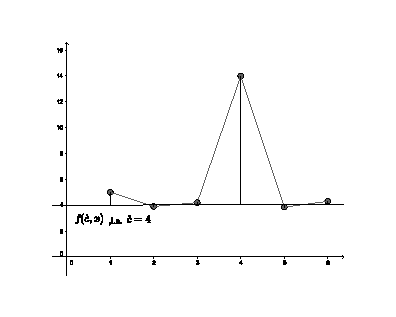
\includegraphics[height=7cm]{IlusExample} }}%
    \qquad
    \subfloat[Illustration of transitions of sign $q_{i}$ between each $\tilde{y}_{i}$]{{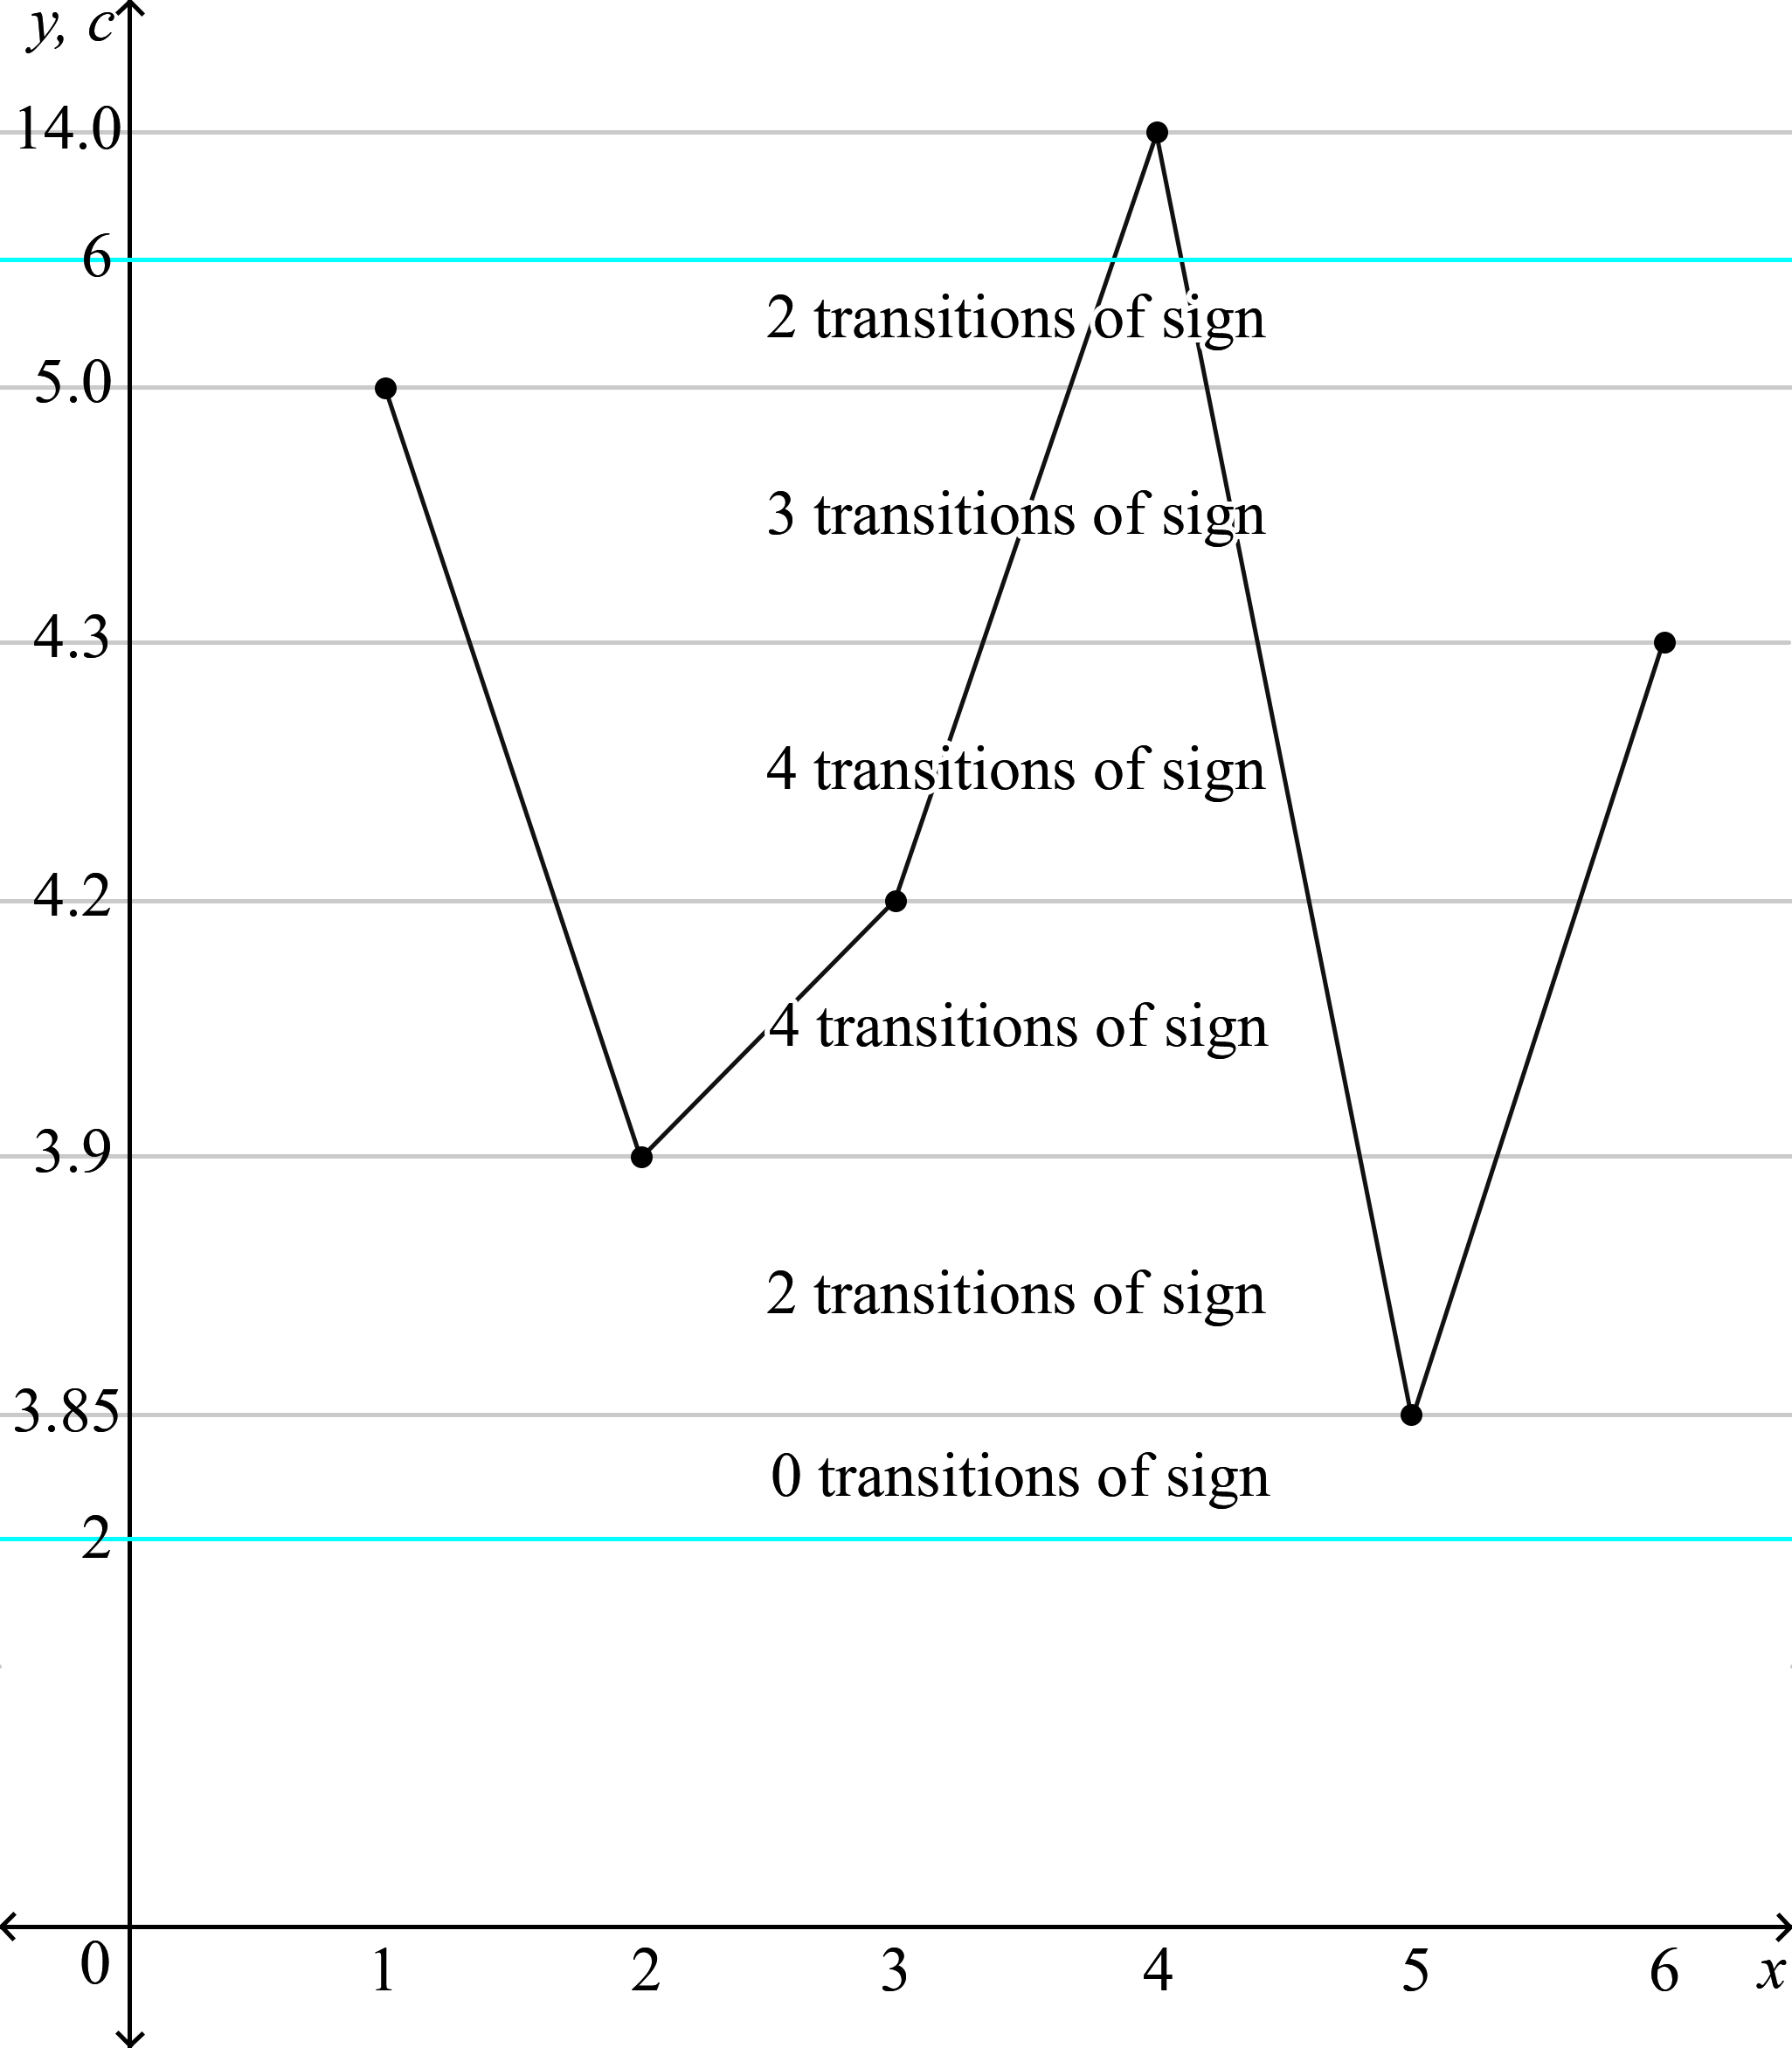
\includegraphics[height=6cm]{examplegraph} }}
    \caption{ }%
    \label{fig:example}%
\end{figure}

\begin{table}[h!]
\caption {Table of values for this example} \label{tab:title} 
\centering
\begin{tabular}{lllll}
$i$ & $x_{i}$ & $f(\dot{c},x_{i})$ & $\xi_{i}$  & $\tilde{y}_{i}=f(\dot{c},x_{i})+\xi_{i}$  \\
1 & 1 & 4      & 1.0   & 5.0   \\
2 & 2 & 4      & -0.1  & 3.9   \\
3 & 3 & 4      & 0.2   & 4.2   \\
4 & 4 & 4      & 10    & 14.0  \\
5 & 5 & 4      & -0.15 & 3.85  \\
0 & 6 & 4      & 0.3   & 4.3  
\end{tabular}
\end{table}
For this example I will use proximity function (\ref{rho2}). \\
\\
As we already know, we can calculate the priori probabilities using (\ref{priori}), where $r=0,1,2,3,4,5$ like so:
\begin{gather*}
p_{0}= \frac{1}{32}; \ p_{1}= \frac{5}{32}; \ p_{2}= \frac{10}{32}; \ p_{3}= \frac{10}{32}; \ p_{4}= \frac{5}{32}; \ p_{5}= \frac{1}{32}
\end{gather*}
But can only have certain values: $r=0,2,3,4$. And ,so 
\begin{gather*}
s=p_{0}+p_{2}+p_{3}+p_{4}= \frac{1}{32} + \frac{10}{32} + \frac{10}{32} + \frac{5}{32} = \frac{26}{32}.
\end{gather*}
So, to calculate the posteriori probabilities
\begin{eqnarray*}
P_{0}^{*} &=& P_{0}: \frac{26}{32} = \frac{1}{32} : \frac{26}{32} = \frac{1}{26} \\
P_{1}^{*} &=& 0 \\
P_{2}^{*} &=& P_{2}: \frac{26}{32} = \frac{10}{32} : \frac{26}{32} = \frac{10}{26} \\
P_{3}^{*} &=& P_{3}: \frac{26}{32} = \frac{10}{26} \\
P_{4}^{*} &=& P_{4}: \frac{26}{32} = \frac{5}{32} : \frac{26}{32} = \frac{5}{26} \\
P_{5}^{*} &=& 0
\end{eqnarray*}
Calculating $E(\rho(c^{*},c))$
\begin{gather*}
E(\rho(c^{*},c)) = \int\limits_{2}^{3.85} \underbrace{(c^{*}-c)^{2}}_{\rho(c^{*},c)} \cdot \frac{\overbrace{\frac{1}{26}}^{p_{0}^{*}}}{\underbrace{3.85-2}_{\text{similar to }\mu(D_{0})}} \mathrm{d}c \ + \int\limits_{3.9}^{4.3} (c^{*}-c)^{2} \cdot \frac{\frac{5}{26}}{4.3-3.9} \mathrm{d}c \
+ \int\limits_{4.3}^{5.0} (c^{*}-c)^{2} \cdot \frac{\frac{10}{26}}{5.0-4.3} \mathrm{d}c \\
+ \ 1.05 \cdot \left( \ \int\limits_{3.85}^{3.9} (c^{*}-c)^{2} \cdot \frac{10}{26} \mathrm{d}c + \
\int\limits_{5.0}^{6.0} (c^{*}-c)^{2} \cdot \frac{10}{26} \mathrm{d}c \right) \\
=(c^{*})^{2} \cdot c - c^{*} \cdot c^{2} + \frac{1}{3} c^{3}
\end{gather*}
Taking into account that later we will want to find the derivative $\frac{\mathrm{d}E(\rho(c^{*},c))}{\mathrm{d}c^{*}}$, we can omit the summand $\frac{1}{3} c^{3}$ as it is a constant, and the derivative of a constant is zero. Let's continue.
\begin{eqnarray*}
E(\rho(c^{*},c)) = 0.045 &\left[ (c^{*})^{2} \cdot c - c^{*} \cdot c^{2} \right]&_{2}^{3.85}  \\
+ 7.323  &\left[ (c^{*})^{2} \cdot c - c^{*} \cdot c^{2} \right]&_{3.85}^{3.9} \\
+ 0.481 &\left[ (c^{*})^{2} \cdot c - c^{*} \cdot c^{2} \right]&_{3.9}^{4.3}  \\
+ 0.549 &\left[ (c^{*})^{2} \cdot c - c^{*} \cdot c^{2} \right]&_{4.3}^{5.0}  \\
+ 0.366 &\left[ (c^{*})^{2} \cdot c - c^{*} \cdot c^{2} \right]&_{5.0}^{6.0}  \\
= &1.361(c^{*})^{2}-12.061c^{*}&
\end{eqnarray*}

\begin{eqnarray*}
\frac{\mathrm{d}E(\rho(c^{*},c))}{\mathrm{d}c^{*}} &=& 2.722c^{*}-12.061 = 0 \\
c^{*} &=& \frac{12.061}{2.722} = 4.431
\end{eqnarray*}
Seeing that $\dot{c} = 4.0$, we finally calculate $\rho$ using this method
\begin{equation*}
\rho = |4.431-4.0| = 0.431
\end{equation*}
I.e. the error made by this method is 0.431. Now let's see what kind of error will the Least Square Method give:
\begin{gather*}
Using Least Square Method \\
\phi(c^{*})= \sum\limits_{i=1}^{6}(\tilde{y}_{i}-c^{*})^{2} \longrightarrow min \\
\phi(c^{*})= \sum\limits_{i=1}^{6}(\tilde{y}_{i}^{2}-2 \tilde{y}_{i}c^{*} + (c^{*})^{2}) \\
\frac{\mathrm{d}\phi(c^{*})}{\mathrm{d}c^{*}} =  \sum\limits_{i=1}^{6}(0 -\cancel{2} \tilde{y}_{i} +\cancel{2} c^{*}) = 0 \\
\sum\limits_{i=1}^{6}c^{*} = \sum\limits_{i=1}^{6} \tilde{y}_{i} \\
6 \cdot c^{*} = \sum\limits_{i=1}^{6} \tilde{y}_{i} = 35.25 \\
c^{*} = \frac{35.25}{6} = 5.875 \\
\text{And so the error } \rho = 1.875
\end{gather*}
LSM gives a bigger error because in it deviations are squared \footnote{\cite{Plackett_1950}}, and therefore large derivations are weighted more heavily. Because this example shows, that in the case of significant non-compliance to condition $E(\xi)=0$, my method is notably superior to LSM, and because of the limited format of this IA, I will not include further solutions that used LSM. %You may refer to (*) in the apendix for more such results.
 Back to the theory.\\
\\
\end{subsection}
Let the proximity $\rho(c^{*},c)$ in (\ref{mathexpectancy}), be taken in the form (\ref{rho2}). Then the following simplification takes place.
\begin{gather}
\nonumber
E(\rho(c^{*},\dot{c}))=\sum\limits_{r \in I} \frac{p_{r}^{*}}{\mu(D_{r})} \int\limits_{D_{r}}\sum\limits_{j=1}^{m} \left( c_{j}^{*}-c_{j} \right)^{2}\mathrm{d}c_{1}\mathrm{d}c_{2}\dots \mathrm{d}c_{m} = \\
\nonumber
\textit{expanding} \left( c_{j}^{*}-c_{j} \right)^{2} \\
\nonumber
\sum\limits_{r \in I} \frac{p_{r}^{*}}{\mu(D_{r})} \sum\limits_{j=1}^{m} \left[ (c_{j}^{*})^{2} \underbrace{\int\limits_{D_{r}} \mathrm{d}c_{1}\mathrm{d}c_{2}\dots \mathrm{d}c_{m}}_{{=\mu(D_{r})}} - 2c_{j}^{*} \int\limits_{D_{r}} c_{j} \  \mathrm{d}c_{1}\mathrm{d}c_{2}\dots \mathrm{d}c_{m} + \int\limits_{D_{r}} c_{j}^{2} \  \mathrm{d}c_{1}\mathrm{d}c_{2}\dots \mathrm{d}c_{m}\right]= \\
\nonumber
\sum\limits_{j=1}^{m} \left( \sum\limits_{r \in I} \frac{p_{r}^{*}}{\mu(D_{r})} \left[ (c_{j}^{*})^{2} \mu(D_{r})-2c_{j}^{*} \int\limits_{D_{r}} c_{j} \  \mathrm{d}c_{1}\mathrm{d}c_{2}\dots \mathrm{d}c_{m} + \int\limits_{D_{r}} c_{j}^{2} \  \mathrm{d}c_{1}\mathrm{d}c_{2}\dots \mathrm{d}c_{m} \right] \right) = \\ 
\sum\limits_{j=1}^{m} \left( (c_{j}^{*})^{2} \cancel{\mu(D_{r})} \underbrace{\sum\limits_{r \in I} \frac{p_{r}^{*}}{\cancel{\mu(D_{r})}}}_{\sum\limits_{r \in I}p_{r}^{*} = 1} - 2c_{j}^{*} \sum\limits_{r \in I}\frac{p_{r}^{*}}{\mu(D_{r})} \int\limits_{D_{r}} c_{j} \  \mathrm{d}c_{1}\mathrm{d}c_{2}\dots \mathrm{d}c_{m} + \sum\limits_{r \in I}\frac{p_{r}^{*}}{\mu(D_{r})} \int\limits_{D_{r}} c_{j}^{2} \  \mathrm{d}c_{1}\mathrm{d}c_{2}\dots \mathrm{d}c_{m} \right)
\end{gather}
And finally:
\begin{equation}
E(\rho(c^{*},\dot{c}))= \sum\limits_{j=1}^{m} \left( (c_{j}^{*})^{2} - 2c_{j}^{*} \sum\limits_{r \in I} p_{r}^{*} \frac{\int\limits_{D_{r}} c_{j} \  \mathrm{d}c_{1}\mathrm{d}c_{2}\dots \mathrm{d}c_{m}}{\mu(D_{r})} + \underbrace{\sum\limits_{r \in I} p_{r}^{*} \frac{\int\limits_{D_{r}} c_{j}^{2} \  \mathrm{d}c_{1}\mathrm{d}c_{2}\dots \mathrm{d}c_{m}}{\mu(D_{r})}}_{\text{derivative of this with respect to } c_{1}^{*}, c_{2}^{*},\dots,c_{m}^{*} = 0} \right) \label{eq-Erho-simp}
\end{equation}
In order to find the vector $c^{*}$, which provides the minimum of function (\ref{eq-Erho-simp}) and which I will take as the optimal estimate of the unknown vector $\dot{c}$, it is necessary (like in the case with a simple one-parameter function) to take the first partial derivative $\frac{\partial E}{\partial c_{j}^{*}}$ of function (\ref{eq-Erho-simp}) with respect to each variable $c_{j}^{*}$ \footnote{\cite{stewart_2008_deriv}}. After that, equate these derivatives to zero and solve the resulting system of linear equations. In this case, this system splits into $m$ separate linear equation with one variable:
\begin{equation}
2 c_{j}^{*} - 2 \sum\limits_{r \in I} p_{r}^{*}\frac{\int\limits_{D_{r}} c_{j}\mathrm{d}c_{1}\mathrm{d}c_{2}\dots\mathrm{d}c_{m}}{\mu(D_{r})} , \quad j = 1,2,\dots,m.
\end{equation}
These equations have the following solutions:
\begin{equation}
c_{j}^{*} = \sum\limits_{r \in I} p_{r}^{*} \bar{c}_{(j,r)}, \quad j = 1,2,\dots,m, \label{eq-solutions-to-cj*}
\end{equation}
where
\begin{equation}
\bar{c}_{(j,r)} = \frac{\int\limits_{D_{r}} c_{j}\mathrm{d}c_{1}\mathrm{d}c_{2}\dots\mathrm{d}c_{m}}{\mu(D_{r})}. \label{eq-cbar}
\end{equation}
\\
Note that the equations (\ref{eq-solutions-to-cj*}) and (\ref{eq-cbar}) - even though in some other notations - are the put forward in Regg-Med-Noise.\\
\\
From the point of view of practical realisation of my algorithm, that is based of formulae (\ref{eq-solutions-to-cj*}),(\ref{eq-cbar}), I can ask two questions: 1. Is it possible to derive a simple method of constructing the sets $D_{r}$; 2. Is it possible to derive a simple method of calculation the integrals of those sets $D_{r}$, which appear in the RHS of (\ref{eq-cbar}). What a geometrical construction (Figure (omitted)) has shown me, is that even in the case where $m=2$ and $n=10$, the regions $D_{r}$ have a relatively complicated geometry (some multi-peaked star-like shapes). However, this problem can be solved with the principal of the 'Gordian knot' - refuse to work with directly with sets $D_{r}$, but instead, to use their point (grid) approximation (even without describing these sets concretely) and use an analog of (\ref{eq-solutions-to-cj*}).\\
\\
The essence of this suggested method of thinking is as follows. Define $k(1),k(2),\dots,k(m)$ as some quite large real values, and a $m$-dimensional parallelepiped
\begin{equation}
W=\{ c:c_{j}^{(\text{min)}} \leq c_{j} \leq c_{j}^{(\text{max)}}, \quad j=1,2,\dots,m \}\subset \boldsymbol{R}^{m}
\end{equation}
which contains the set $D$ (if the set $D$ itself is a parallelepiped, then $W=D$). Cover this parallelepiped with a dense grid $\Gamma$ with
\begin{equation}
L = \prod\limits_{t=1}^{m}k(t)
\end{equation}
number of nodes $c^{(l)} = (c_{1}^{(l)},(c_{2}^{(l)},\dots,c_{m}^{(l)}),\quad l=1,2,\dots,L$, where each coordinate $c_{j}^{(l)}, \quad j=1,2,\dots,m,$ could independently from all the other $m-1$ coordinates (note that $m-1$ does not refer to sets of coordinates) assume one of $k(j)$ of values
\begin{equation}
c_{j}=c_{j}^{(\text{min})} + \frac{c_{j}^{(\text{max})}-c_{j}^{(\text{min})}}{k(j)}(t-\frac{1}{2}), \quad t=1,2,\dots,k(j).
\end{equation}
Parallel to grid $\Gamma$ implement the system $A$ of parallelepipeds $W_{l} \subset \boldsymbol{R}^{m}, \quad l=1,2,\dots,L,$ the centres of which are their nodes with sides
\begin{gather}
h_{j} = \frac{(c_{j}^{(\text{max})}-c_{j}^{(\text{min})})}{k(j)}: \\
W_{l} = \lbrace c=(c_{1},c_{2},\dots,c_{m}):c_{j}^{(l)}-\frac{1}{2} h_{j} \leq c_{j} \leq c_{j}^{(l)}+\frac{1}{2} h_{j}, \quad j=1,2,\dots,m \rbrace .
\end{gather}
These parallelepipeds form the surface of the parallelepiped W. Now we have to chose from the defined $L$ nodes those, the ones who belong to the set $D$. Let $L_{0}$ be the quantity of the chosen nodes. Renumber the chosen nodes, by assigning the first $L_{0}$ numbers $l$ to them. \\
\\
For each $l=1,2,\dots,L_{0}$ find elements of $q_{i}(c^{(l)}), \quad i=1,2,\dots,n$ of sequence (\ref{sequence}), and based on their values, using (\ref{eq-values-of-q}), calculate the number $r$ of transition of sign of elements of (\ref{sequence}). Let $J_{r}, \quad r=0,1,\dots,n-1$ be the set of numbers $l$ of chosen nodes $c^{(l)}$ providing $r$ transitions of sign, and $|J_{r}|$ - the number of nodes giving that many transitions. In this way, without directly constructing the sub-sets $D_{r}$, I approximate each of them with the union
\begin{equation}
\tilde{D}_{r} = \bigcup_{l \in J_{r}} W_{l}.
\end{equation}
\\
It is clear, that the assumption, that all vectors $c$, belonging to the parallelepiped $W_{l}$, will provide the same number of transitions of sign as the center $c^{l}$ of the parallelepiped, will only be incorrect for those parallelepipeds $W_{l}$, and do not completely belong to some one sub-set $D_{r}$. But with a dense grid $\Gamma$, and respectively, quite small-sized parallelepipeds $W_{(l)}$, the percent of such 'debatable' parallelepipeds compared to their general number $L_{0}$ will be quite small (so, in figure (omitted), when $m=2$, these 'debatable' parallelepipeds are positioned along the lines, and the 'non-debatable' - in the areas). In addition, the error resulting from classification of such 'debatable' parallelepipeds $W_{l}$ completely to some set $D_{r}$, will get (mostly) redeemed/repaid. Summing up all these arguments, it can be said, that the approximations of sets $D_{r}$, with the union of relatively 'small' parallelepipeds will give a good  approximation of the mathematical expectancy (\ref{mathexpectancy}) of error in estimation of parameters of a studies functional dependence:
\begin{gather}
\nonumber
E(\rho_{2}(c^{*},c)) \approx \sum\limits_{r \in I} \frac{p_{r}^{*}}{\mu(\tilde{D}_{r})} \int\limits_{\tilde{D}_{r}} \sum\limits_{j=1}^{m}(c_{j}^{*}-c_{j})^{2}\mathrm{d}c_{1}\mathrm{d}c_{2}\dots \mathrm{d}c_{m} = \\
\nonumber 
\text{(integral with limit } D_{r} \text{ can be split as the sum of integrals with limit } W_{l} \text{)}\\
\sum\limits_{r \in I} \frac{p_{r}^{*}}{\mu(\tilde{D}_{r})} \sum\limits_{l \in J_{r}} \  \int\limits_{W_{l}} \sum\limits_{j=1}^{m}(c_{j}^{*}-c_{j})^{2}\mathrm{d}c_{1}\mathrm{d}c_{2}\dots \mathrm{d}c_{m} = \\
\nonumber
\text{(the sum } \sum_{j=1}^{m} \text{ is facrotised out)} \\
\nonumber
\sum\limits_{j=1}^{m}  \left[ \sum\limits_{r \in I} \frac{p_{r}^{*}}{\mu(\tilde{D}_{r})} \left( \sum\limits_{l \in J_{r}} \ \int\limits_{W_{l}} ((c_{j}^{*})^{2}-2c_{j}^{*}c_{j}+c_{j}^{2}) \right) \mathrm{d}c_{1}\mathrm{d}c_{2}\dots \mathrm{d}c_{m} \right] = \\
\nonumber
\text{(expanding } ((c_{j}^{*})^{2}-2c_{j}^{*}c_{j}+c_{j}^{2}) \text{)}\\
\sum\limits_{j=1}^{m}  \left[ \sum\limits_{r \in I} \frac{p_{r}^{*}}{\mu(\tilde{D}_{r})} \left( \sum\limits_{l \in J_{r}} \left[ (c_{j}^{*})^{2} \mu(W_{(l)}) - 2c_{j}^{*} \int\limits_{W_{l}} c_{j} \mathrm{d}c_{1}\mathrm{d}c_{2}\dots \mathrm{d}c_{m} + \int\limits_{W_{l}} c_{j}^{2} \mathrm{d}c_{1}\mathrm{d}c_{2}\dots \mathrm{d}c_{m} \right] \right) \right]. \label{eq-simplification-chain}
\end{gather}
If in a multiple integral, the limits of integration for each variable are given by other variables, then this multiple integral is equal to the product of included in it, one-dimensional integrals \footnote{\cite{stewart_2008_int}}. Now, if we define coordinates of the edges of $W_{l}$ as $c_{j}^{(l)} - 0.5h_{j} = a(j,l)$ and $c_{j}^{(l)} + 0.5h_{j} = b(j,l)$ then it is not hard to be sure that 
\begin{equation}
\frac{1}{\mu(W_{l})} \int\limits_{W_l} c_{j} \mathrm{d} c_{1} \mathrm{d} c_{2} \ldots  \mathrm{d} c_{m} 
	= \dfrac{1}{\prod\limits_{s=1}^{m}h_{s}}
	\left( \  \int\limits_{b(j,l)}^{a(j,l)} c_{j}  \mathrm{d} c_{j}\right) 
	\prod_{\substack{s=1\\ (s\ne j)}}^m \ 
	\int\limits_{a(s,l)}^{b(s,l)} \!  \mathrm{d} c_{s} 
	= c_{j}^{(l)}.
\end{equation}
If in addition we accept that
\begin{gather}
\sum\limits_{r \in I} p_{r}^{*} =1, \\
\sum\limits_{l \in J_{r}} \mu(W_{l}) =\mu(\tilde{D}_{r}), \\
\mu(W_{l}) \equiv \prod\limits_{j=1}^{m}h_{j},
\end{gather}
then the simplification chain (\ref{eq-simplification-chain}) could be continued
\begin{gather}
\nonumber
E(\rho_{2}(c^{*},c)) \approx \sum\limits_{j=1}^{m}  \left[ \sum\limits_{r \in I} \frac{p_{r}^{*}}{\mu(\tilde{D}_{r})} \left( \sum\limits_{l \in J_{r}} \left[ (c_{j}^{*})^{2} \mu(W_{l}) - 2c_{j}^{*} \mu(W_{l}) c_{j}^{(l)} + \int\limits_{W_{l}} c_{j}^{2} \mathrm{d}c_{1} \mathrm{d}c_{2} \dots \mathrm{d}c_{m} \right] \right) \right] = 
\end{gather}
\begin{gather}
\nonumber
\text{( middle step: } \sum_{l \in J_{r}}^{m}(c_{j}^{*})^{2} \mu(W_{l}) = (c_{j}^{*})^{2} \underbrace{\sum_{l \in J_{r}} \mu(W_{l})}_{=\mu(\tilde{D}_{r})} = (c_{j}^{*})^{2} \mu(\tilde{D}_{r}) \text{ )} \\
\nonumber
\sum\limits_{j=1}^{m} \left[  (c_{j}^{*})^{2}  \sum\limits_{r \in I} p_{r}^{*}  - 2c_{j}^{*}  \sum\limits_{r \in I} \frac{p_{r}^{*}}{\mu(\tilde{D}_{r})} \sum\limits_{l \in J_{r}} \mu(W_{l})  c_{j}^{(l)}  + \sum\limits_{r \in I} \frac{p_{r}^{*}}{\mu(\tilde{D}_{r})} \sum\limits_{l \in J_{r}} \ \int\limits_{W_{l}} c_{j}^{2}  \mathrm{d}c_{1} \mathrm{d}c_{2} \dots \mathrm{d}c_{m} \right] = \\
\nonumber
\text{( middle step: } \sum_{r \in I} (c_{j}^{*})^{2} \frac{p_{r}^{*}}{\cancel{\mu(\tilde{D}_{r})}} \cancel{\mu(\tilde{D}_{r})} = (c_{j}^{*})^{2} \underbrace{\sum_{r \in I} p_{j}^{*}}_{=1} = (c_{j}^{*})^{2} \text{ )}\\
\nonumber
\sum\limits_{j=1}^{m} \left[  (c_{j}^{*})^{2} - 2c_{j}^{*} \sum\limits_{r \in I} p_{j}^{*} \frac{1}{\sum\limits_{l \in J_{r}} \mu(W_{l})} \sum\limits_{l \in J_{r}} \mu(W_{j}) c_{j}^{(l)} +  \sum\limits_{r \in I} \frac{p_{r}^{*}}{\mu(\tilde{D}_{r})} \sum\limits_{l \in J_{r}} \ \int\limits_{W_{l}} c_{j}^{2}  \mathrm{d}c_{1} \mathrm{d}c_{2} \dots \mathrm{d}c_{m} \right] = \\
\nonumber
\sum\limits_{j=1}^{m}  \left[    (c_{j}^{*})^{2} - 2c_{j}^{*} \sum\limits_{r \in I} p_{j}^{*} \frac{1}{\left| J_{r} \right| \prod\limits_{s=1}^{m} h_{s}} \sum\limits_{l \in J_{r}} \left( \prod_{s=1}^{m} h_{s} \right) c_{j}^{(l)} +  \sum\limits_{r \in I} \frac{p_{r}^{*}}{\mu(\tilde{D}_{r})} \sum\limits_{l \in J_{r}} \ \int\limits_{W_{l}} c_{j}^{2}  \mathrm{d}c_{1} \mathrm{d}c_{2} \dots \mathrm{d}c_{m} \right] = \\
\sum\limits_{j=1}^{m} \left[ c_{j}^{*})^{2} - 2c_{j}^{*} \sum\limits_{r \in I} \frac{p_{j}^{*}}{ \left| J_{r} \right|} \sum\limits_{l \in J_{r}} c_{j}^{(l)} + \sum\limits_{r \in I} \frac{p_{r}^{*}}{\mu(\tilde{D}_{r})} \sum\limits_{l \in J_{r}} \ \int\limits_{W_{l}} c_{j}^{2}  \mathrm{d}c_{1} \mathrm{d}c_{2} \dots \mathrm{d}c_{m} \right]. \label{eq-final-simplification}
\end{gather}
In order to find vector $c^{*}$, which provides the minimum estimate mathematical expectation (\ref{eq-final-simplification}) of error in the approximation of unknown true parameters of the functional dependence in question, and therefore also of vector $\dot{c}$, we take the same steps as in the case when we calculated the minimum of function (\ref{eq-Erho-simp}). Taking into account, that the last, third, summand in (\ref{eq-final-simplification}) does not contain 
any variables $c_{j}^{*}$ (which are being optimised), its derivative is again equal to zero, we find its partial derivatives:
\begin{equation}
\frac{\partial E (\rho_{2}(c^{*},c))}{\partial c_{j}^{*}} \approx 2c_{j}^{*} - 2 \sum\limits_{r \in I} \frac{p_{r}^{*}}{\left| J_{r} \right|} \sum\limits_{l \in J_{r}} c_{j}^{(l)}, \quad j=1,2,\dots,m. \label{eq-partial}
\end{equation}
Equating these partial derivatives (\ref{eq-partial}) to zero we get, and therefore conclude with:
\begin{equation}
c_{j}^{*} = \sum\limits_{r \in I} \frac{p_{r}^{*}}{\left| J_{r} \right|} \sum\limits_{l \in J_{r}} c_{j}^{(l)}, \quad j=1,2,\dots,m. \label{eq-final}
\end{equation}
This equation (\ref{eq-final}) is the one used in calculations of approximate values of the optimised vector $c^{*}$ in my custom software, the trails of which are later in this document.\\
\\
Now, let's compare reviousy suggested in Regg-Med-Noise equations (\ref{eq-solutions-to-cj*}) and (\ref{eq-cbar}) with the suggested equation (\ref{eq-final}). The superiority of the later is shown in that: 1. it does not require the direct construction of sub-sets $D_{r}$
, which in fact are quite complex convex polyhedrons in $\boldsymbol{R}^{m}$ dimensions. Therefore 2. this equation does not require the expansive calculation of multiple integrals found in (\ref{eq-solutions-to-cj*}) and (\ref{eq-cbar}).  In Regg-Med-Noise there is one more problem at hand: even a polygon, not to mention a polyhedron, can not be defined only by its vertexes (those could be connected with line segments in not just one way). The algorithm proposed in this IA to estimate the optimal parameters $c^{*}$, only requires the regular (evenly distributed) surface of set $D$, for the nodes of which the only thing left to do is evaluate the elements of the sequence  \ref{sequence}.

\section{Algorithm trials}
Now that the method that will be used is finalized, testing it is a necessity. First, to show that this method gives better estimates than others (in this case LSM), multiple sets of 'experimental' data with pseudo-random errors of varying intensities were estimated using the method derived here and LSM. Both methods ran through those sets two times, with differing intensities \footnote{Intensity, factually is a positive value used to vertically stretch 'experimental values' about the true functional dependency, in the program used to calculate these approximations.}. The true function in this case had only two parameters $c_{1}^{*}$ and $c_{2}^{*}$, which equal 2.0 and 0.5 respectably, making the true function $y=0,5x + 2$. Note that the pseudo-random error values lie between 3 and -3 under the law of normal distribution.
\begin{table}[h!]
\centering
\caption{Algorithm approximations of sets of data using method derived here}
\label{my-label}
\begin{tabular}{|c|r|r|r|r|r|r|r|r|}
\multirow{2}{*}{sets} & \multicolumn{4}{c|}{intensity=0.15}                                                                                                            & \multicolumn{4}{c|}{intensity=0.3}                                                                                                             \\
                      & \multicolumn{1}{c|}{$c_{1}^{*}$} & \multicolumn{1}{c|}{$c_{2}^{*}$} & \multicolumn{1}{c|}{factual error} & \multicolumn{1}{c|}{extected error} & \multicolumn{1}{c|}{$c_{1}^{*}$} & \multicolumn{1}{c|}{$c_{2}^{*}$} & \multicolumn{1}{c|}{factual error} & \multicolumn{1}{c|}{extected error} \\
1                     & 2.085                            & 0.343                            & 0.032                              & 0.054                               & 2.125                            & 0.333                            & 0.044                              & 0.106                               \\
2                     & 2.085                            & 0.525                            & 0.008                              & 0.074                               & 2.125                            & 0.586                            & 0.211                              & 0.327                               \\
3                     & 1.915                            & 0.667                            & 0.035                              & 0.066                               & 1.870                            & 0.697                            & 0.054                              & 0.119                               \\
4                     & 2.065                            & 0.515                            & 0.004                              & 0.057                               & 2.136                            & 0.535                            & 0.019                              & 0.094                               \\
5                     & 2.166                            & 0.242                            & 0.093                              & 0.035                               & 2.236                            & 0.253                            & 0.117                              & 0.064                               \\
average               & 2.063                            & 0.458                            & 0.034                              & 0.057                               & 2.085                            & 0.479                            & 0.089                              & 0.142                              
\end{tabular}
\end{table}
\begin{table}[h!]
\centering
\caption{Algorithm approximations of sets of distorted data using method derived here}
\label{my-label}
\begin{tabular}{|c|r|r|r|r|r|r|r|r|}
\multirow{2}{*}{\begin{tabular}[c]{@{}c@{}}dist. \\ sets \end{tabular}} & \multicolumn{4}{c|}{intensity=0.15}                                                                                                            & \multicolumn{4}{c|}{intensity=0.3}                                                                                                             \\
                                                                            & \multicolumn{1}{c|}{$c_{1}^{*}$} & \multicolumn{1}{c|}{$c_{2}^{*}$} & \multicolumn{1}{c|}{factual error} & \multicolumn{1}{c|}{extected error} & \multicolumn{1}{c|}{$c_{1}^{*}$} & \multicolumn{1}{c|}{$c_{2}^{*}$} & \multicolumn{1}{c|}{factual error} & \multicolumn{1}{c|}{extected error} \\
1                                                                           & 2.085                            & 0.343                            & 0.038                              & 0.054                               & 2.125                            & 0.333                            & 0.044                              & 0.106                               \\
2                                                                           & 2.085                            & 0.525                            & 0.008                              & 0.074                               & 2.156                            & 0.556                            & 0.027                              & 0.098                               \\
3                                                                           & 1.915                            & 0.667                            & 0.035                              & 0.066                               & 1.974                            & 0.697                            & 0.055                              & 0.120                               \\
4                                                                           & 2.065                            & 0.515                            & 0.004                              & 0.057                               & 2.146                            & 0.535                            & 0.022                              & 0.097                               \\
5                                                                           & 2.166                            & 0.242                            & 0.094                              & 0.035                               & 2.236                            & 0.252                            & 0.117                              & 0.064                               \\
average                                                                     & 2.063                            & 0.458                            & 0.179                              & 0.057                               & 2.127                            & 0.475                            & 0.065                              & 0.097                              
\end{tabular}
\end{table}
\begin{table}[h!]
\centering
\caption{Algorithm approximations of sets of data using LSM}
\label{my-label}
\begin{tabular}{|c|r|r|r|r|r|r|}
\multirow{2}{*}{\begin{tabular}[c]{@{}c@{}}sets\\ (LSM)\end{tabular}} & \multicolumn{3}{c|}{intensity=0.15}                                                                      & \multicolumn{3}{c|}{intensity=0.3}                                                                       \\
                                                                      & \multicolumn{1}{c|}{$c_{1}^{*}$} & \multicolumn{1}{c|}{$c_{2}^{*}$} & \multicolumn{1}{c|}{factual error} & \multicolumn{1}{c|}{$c_{1}^{*}$} & \multicolumn{1}{c|}{$c_{2}^{*}$} & \multicolumn{1}{c|}{factual error} \\
1                                                                     & 2.069                            & 0.361                            & 0.208                              & 2.139                            & 0.224                            & 0.417                              \\
2                                                                     & 2.121                            & 0.382                            & 0.239                              & 2.242                            & 0.264                            & 0.477                              \\
3                                                                     & 2.031                            & 0.478                            & 0.052                              & 2.061                            & 0.457                            & 0.103                              \\
4                                                                     & 2.060                            & 0.480                            & 0.081                              & 2.121                            & 0.459                            & 0.161                              \\
5                                                                     & 2.136                            & 0.294                            & 0.341                              & 2.271                            & 0.088                            & 0.683                              \\
average                                                               & 2.083                            & 0.399                            & 0.186                              & 2.167                            & 0.298                            & 0.288                             
\end{tabular}
\end{table}
\begin{table}[h!]
\centering
\caption{Algorithm approximations of sets of distorted data using LSM}
\label{my-label}
\begin{tabular}{|c|r|r|r|r|r|r|}
\multirow{2}{*}{\begin{tabular}[c]{@{}c@{}}dist. sets\\ (LSM)\end{tabular}} & \multicolumn{3}{c|}{intensity=0.15}                                                                      & \multicolumn{3}{c|}{intensity=0.3}                                                                       \\
                                                                                 & \multicolumn{1}{c|}{$c_{1}^{*}$} & \multicolumn{1}{c|}{$c_{2}^{*}$} & \multicolumn{1}{c|}{factual error} & \multicolumn{1}{c|}{$c_{1}^{*}$} & \multicolumn{1}{c|}{$c_{2}^{*}$} & \multicolumn{1}{c|}{factual error} \\
1                                                                                & 2.069                            & 0.361                            & 0.208                              & 2.253                            & 0.112                            & 0.214                              \\
2                                                                                & 2.121                            & 0.038                            & 0.238                              & 2.286                            & 0.308                            & 0.477                              \\
3                                                                                & 2.030                            & 0.479                            & 0.052                              & 2.164                            & 0.399                            & 0.264                              \\
4                                                                                & 2.060                            & 0.480                            & 0.081                              & 2.264                            & 0.274                            & 0.490                              \\
5                                                                                & 2.136                            & 0.294                            & 0.342                              & 2.341                            & 0.085                            & 0.756                              \\
average                                                                          & 2.083                            & 0.330                            & 0.184                              & 2.262                            & 0.236                            & 0.440                             
\end{tabular}
\end{table}
\\ \\Second, to show that the method is suitable to approximate more complex functional dependences (in this case $y=2x^{3}-2x^{2}+1$), yet again, sets of 'experimental' data with pseudo-random errors of varying intensities were estimated using, now, only this method. Results are shown in the following figures: 
\begin{figure}[h!]%
\centering
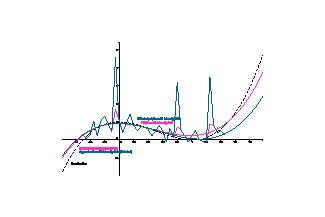
\includegraphics[scale=2.5]{pic-prog2-c-not3}
\caption{Approximation of $y=2x^{3}-2x^{2}+1$ with error intensity=1.0}
\label{fig:results-1}
\end{figure}
\begin{figure}[h!]%
\centering
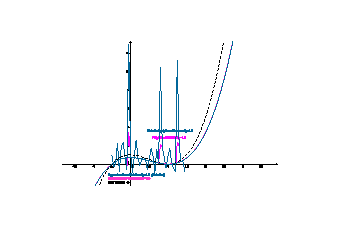
\includegraphics[scale=2.5]{pic-prog2-c-1}
\caption{Approximation of $y=2x^{3}-2x^{2}+1$ with error intensity=0.3}%
\label{fig:results-2}%
\end{figure}
\\You may reefer to additional trials, as well as the source code used for those trials given in the appendix\footnote{Not present in this copy.} of this IA.
\newpage
\section{Conclusion and Reflection}
First of I want to to conclude with mentioning again the conditions in which this method performs best, and subsequently when I would recommend using it. This method approximates, significantly better than LSM per se (and, it could be argued, that better than LAD), in conditions where among measured values $\title{y}_{i}$ there is a significant percentage of such of those values that their absolute value is relatively small (and therefore they are close to the studied functional dependence). We can't know which of them are so, and we don't have to, we just need to know that such values of $\title{y}_{i}$ exist. Said that, some values $\title{y}_{i}$ can peak quite significantly in one of the signs (+ve or -ve), without the approximation begin significantly affected. It is clear, that all conditions in which this method performs best can not be defined (the limited nature of calculation accounts for this), however, the trails given give a good representation of the success of this method.  And thus I have reached my aim. \\
\\
This is to say, that this investigation is far from perfect. Even though begin more constructive than previous work (such as Regg-Med-Noise) done in this topic , there are some holes. For example, the algorithm requires that a finite interval $[\alpha, \beta]$ is given to each parameter estimated, a computer can't run a calculation infinitely. \\
\\
I want to to note that the trials have shown  some results that I have not expected. For example, some individual trails (given in the appendix of this IA) have either unreasonably low of high factual error (error actually made by the method). This could be caused by some random 'layout' of the values of $\title{y}_{i}$ being either in favor or against a good approximation with any method (say when all or close to all absolute values of $\tilde{y}_{i}$ are large) or a bug in my code (but hopefully not that). \\
\\
In spite that, now, after writing and researching for this IA, I know that not only I have questioned the validity of a method of approximation. In it's own way deriving methods of approximation is its own mathematical field. Some methods work better than others in different circumstances. Just like the method described in this IA is suited for use even when there are peaks in the given data, other methods deal with other circumstances, like for example LSM, is suited for circumstances without those peaks. And so, like in most fields in mathematics, this is a continuation from what came before, and could (and should) be continued (by others) to find even better (working in more conditions) algorithms of approximation.



\newpage
\bibliographystyle{apalike}
\bibliography{BIBLIOGRAPHY}

\end{document}

